\subsection{Test Journal: } \label{app:tj_01}

\textbf{Executed by: Martin} \\
\textbf{Date: 18/10/2022}

\subsubsection{Objective}
The objective of this test journal is to document the 1P and 3P frequencies as well as the modes of the WT structure. It is additionally of interest to see how close the frequencies are.

\subsubsection{Background}
The 1P frequency is the rotational frequency of the WT while the 3P frequency is the third multiple of 1P. The second tower mode of a FOWT is located lower than the 3P frequency but very close to the 3P frequency. This may impose problems because resonance can occur if the frequencies come too close.

\subsubsection{Test subject}
The test subject is the V164 8MW wind turbine simulation in VTS.

\subsubsection{Equipment/Software used and test setup}
VTS is used to simulate and Matlab is used to plot the data.

\subsubsection{Test procedure}
Three simulations are plotted. All three simulations has average 14 m/s wind speed. One has regular turbulence, one has very low turbulence and one has normal turbulence and the fore-aft tower damper (FATD) turned off.

\subsubsection{Results and Comments}
Figure \cref{fig:tj1:vfreetomgen} is included to get a general sense of how the turbine is behaving in the three different simulations. The contents of the plot are not the ones of actual interest to this test. The free wind speed is observed in the first subplot. The turbulence for both the baseline and FATDoff plots is obviously much greater than for the baselineNoturb plot. From both the blade pitch angle, rotor speed angular velocity and the generator torque it is very obvious that the turbine is tilting back and forth in the plots where the FATD is turned off.

In \cref{fig:tj1_PSIxVelyVelFFT} a plot of the fft of both the rotor azimuth, tower roll speed and tower pitch speed. The notation here is normal DOF notation. Labels have been placed to more accurately point out the frequencies of interest. The frequency content around 0.3-0.4 Hz is the eigenfrequency of the WT structure. The frequency pins around 0.460-0.483 Hz are the second mode of the WT structure. The pins around 0.520-0.521 Hz are the 3P frequencies. The 1P frequency is very visible from the first subplot around 0.17 Hz. It is quite obvious that indeed the second mode of the tower is quite close to the 3P frequency. 

\begin{figure}[ht]
	\centering
	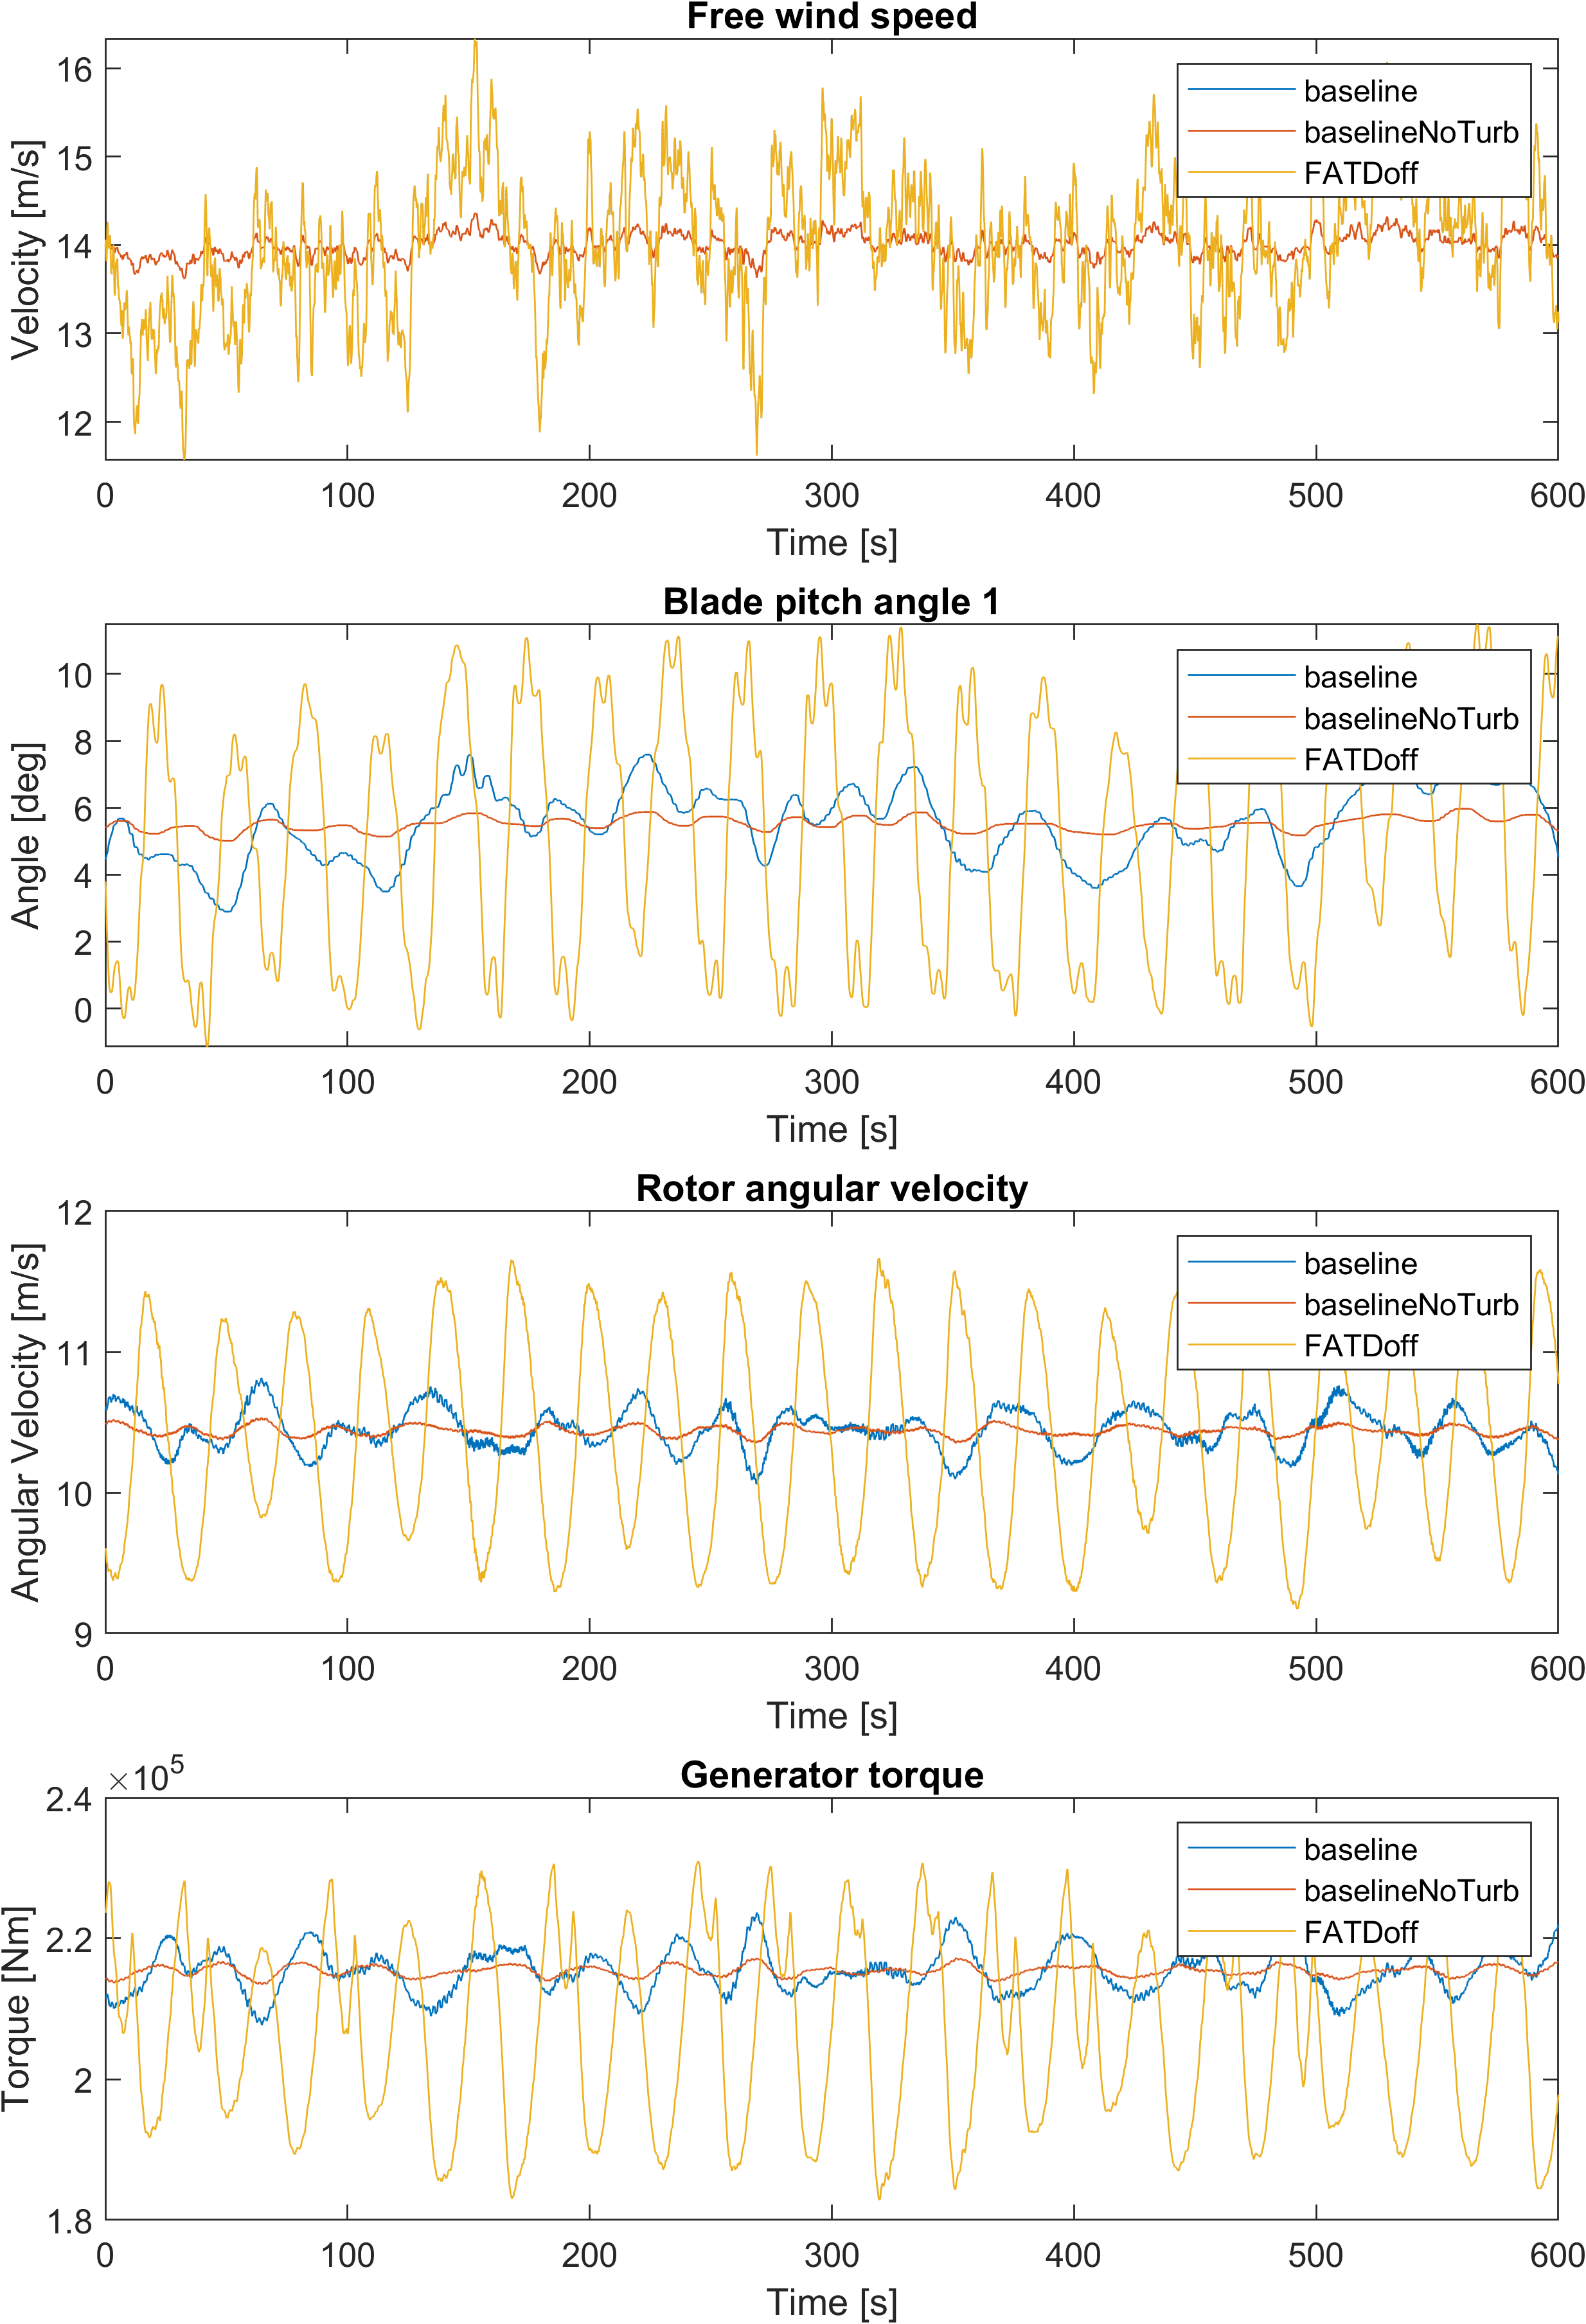
\includegraphics[width=0.8\linewidth]{Graphics/TestResults/tj01/VfreeToMgen.png}
	\caption{Plot of the free wind speed, the first blade pitch, the rotor angular velocity and the generator torque}.
	\label{fig:tj1:vfreetomgen}
\end{figure}

\begin{figure}[ht]
	\centering
	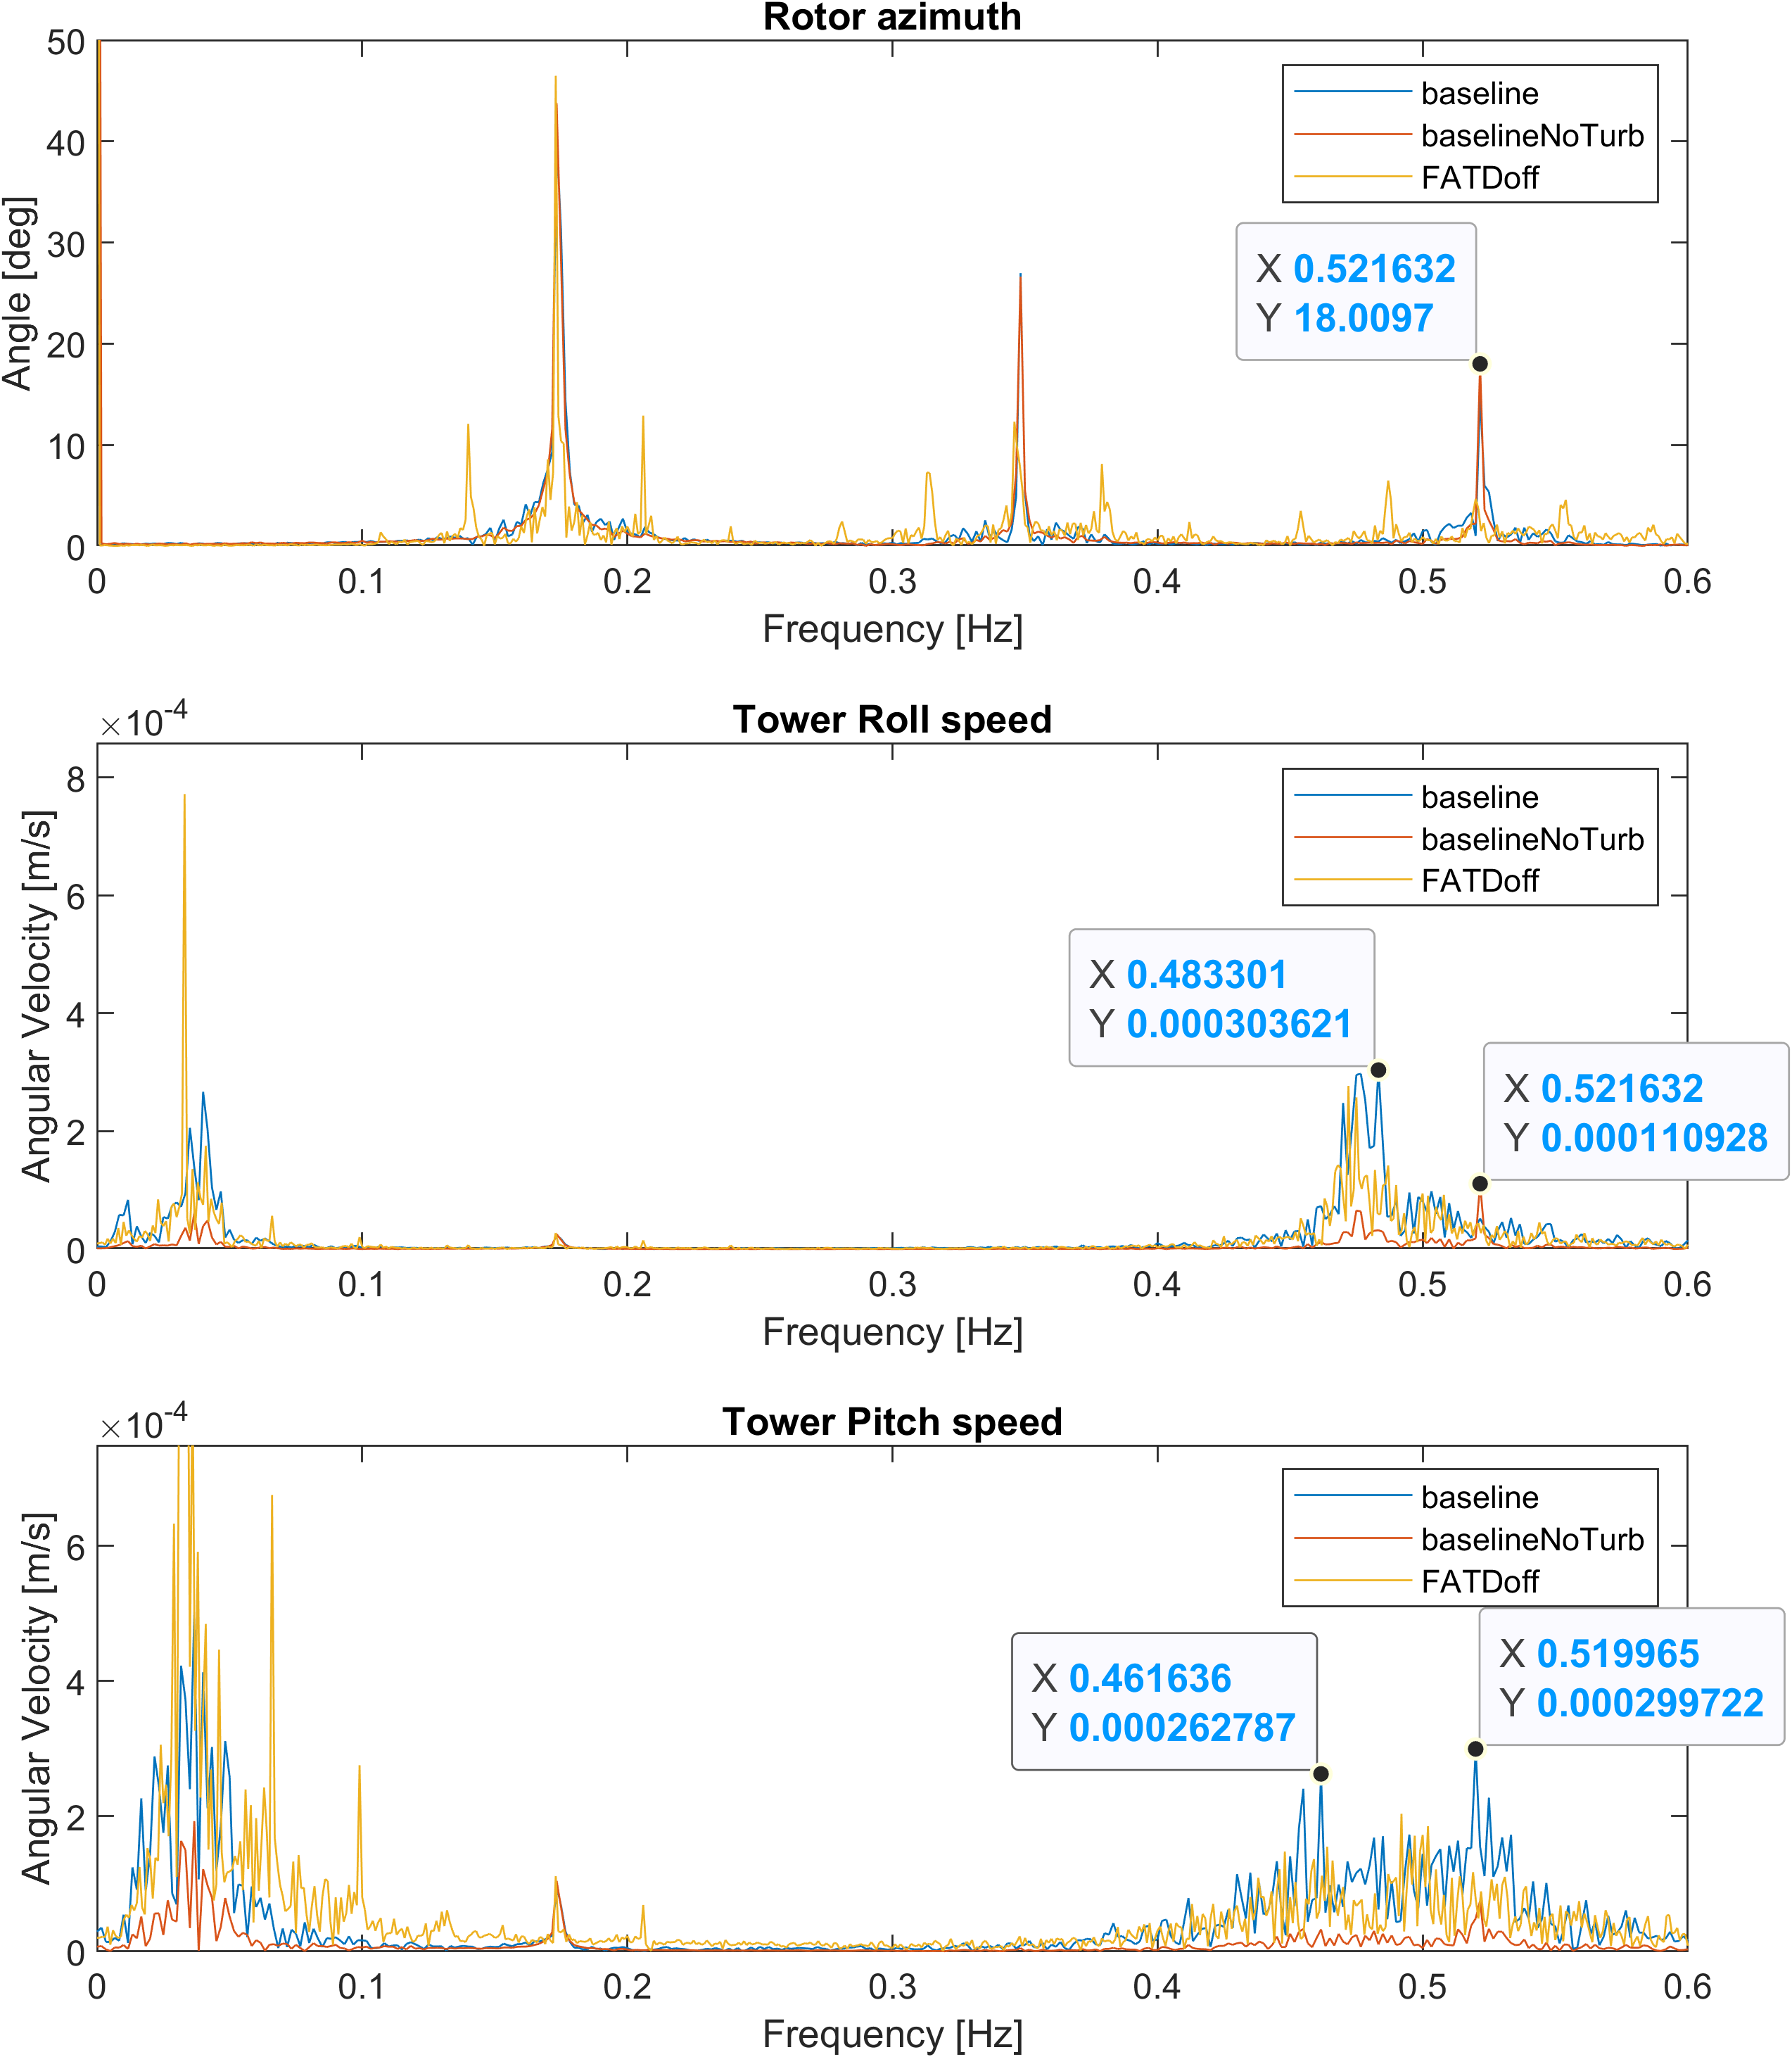
\includegraphics[width=0.8\linewidth]{Graphics/TestResults/tj01/PSIxVelyVelFFT.png}
	\caption{Plot of FFT of the rotor azimuth, tower roll angle and tower pitch angle.}
	\label{fig:tj1_PSIxVelyVelFFT}
\end{figure}
